%% ======================================================================
%% 04d_dron_rampa_bateria.tex -- 3. Modelo (parte 3): por que un dron en la rampa y margen de bateria
%% Cifras: scripts_modelo/rampa.py y scripts_modelo/bateria.py
%% ======================================================================
\subsection{Por qué un dron en la rampa}
\label{sec:porquedron}

La etapa intermedia de AeroTray podría haber sido un cardán motorizado de dos ejes. Esta sección muestra qué aporta el octocóptero en la rampa y con qué costo, a partir de las ecuaciones ya deducidas.

\paragraph{Idea central: un actuador que no empuja contra la base}
Un plato movido por servos fijos a la base, o un cardán motorizado, genera su par \emph{entre} la base y el plato. Por acción y reacción ocurren tres cosas: toda inclinación de la base (la pendiente y los golpes al cruzar los quiebres de la rampa) la debe restar el mismo actuador con su recorrido; esos golpes llegan al plato a través de la transmisión rígida; y la referencia de nivel es la base. El octocóptero sobre la rótula rompe esa cadena. La rótula no transmite par, solo fuerza. El dron genera su par contra el aire y se referencia a la gravedad con su IMU. Por eso la pendiente no entra al plato, y los actuadores quedan separados por escalas: el dron se ocupa de los ángulos grandes y lentos (la pendiente, \SIrange{0}{20}{\degree}, por debajo de \SI{0.3}{\hertz}), y los servos de los ángulos pequeños y rápidos que necesita la bola. Ninguna etapa que reaccione contra la base puede ofrecer esa separación sin gastar recorrido de sus actuadores. A eso se suma una propiedad exclusiva del dron: su empuje es un lastre ajustable (punto~2).

\paragraph{Evidencia con los registros del 18/11}
En los once recorridos grabados ese día el dron iba libre en la rótula a \SI{1300}{\micro\second}. El uso medio del recorrido de los servos fue de 36--57\% en los siete recorridos de rampa y de 43--63\% en los cuatro de llano. El sesgo mediano de los pulsos en la rampa no superó \SI{\pm60}{\micro\second}. Con la bandeja fija a la base, solo nivelar la pendiente de \SI{10}{\degree} habría exigido un sesgo de unos \SI{204}{\micro\second}, es decir, el 93\% del recorrido. Los servos no trabajaron más en la rampa que en el llano: la pendiente no llegó al plato. Una prueba comparativa directa —el ensayo D descrito en la Sección~\ref{sec:metodologia}: recorrer la misma rampa con el dron trabado a la base (\emph{solo servos}) y con el dron libre para comparar uso y saturación de servos, error de la bola y pérdidas— quedó pendiente como trabajo futuro (Sección~\ref{sec:limits}).

\paragraph{1. Nivelación: la pendiente desaparece del plato}
Por \eqref{eq:tilt}, la inclinación absoluta del plato es $\theta+\alpha_y$ y no contiene $\beta$. El octocóptero lleva $\theta$ a cero con su propia IMU, así que los servos solo corrigen la posición de la bola. Con la bandeja fija a la base, la pendiente consumiría $\beta$ de los \SI{\pm10.8}{\degree} de recorrido del plato: en la rampa de \SI{10}{\degree} quedarían \SI{0.8}{\degree} para controlar la bola, y en \SI{20}{\degree} el plato no se podría nivelar. En vuelo estacionario el octocóptero mantuvo el plano de la bandeja a 0,55--1,7$^\circ$ RMS de la horizontal (Sección~\ref{sec:flights}), es decir, deja libre entre el 84 y el 95\% del recorrido de los servos. Un cardán con su propia IMU también podría nivelar, pero lo haría reaccionando contra la base y con un recorrido acotado por sus actuadores; la siguiente función, en cambio, solo la tiene el dron.

\paragraph{2. Descarga de peso: un lastre ajustable}
Sea $f=T/\big((m+m_c)g\big)\in[0,1]$ la fracción del peso del módulo que sostienen los rotores. Mientras $f<1$ el módulo apoya en el tope inferior de la guía \eqref{eq:guide}, y como se nivela, su empuje es vertical en $\{W\}$. En el balance de momentos de \eqref{eq:tip} el empuje equivale entonces a reducir la masa del módulo en la rótula a $(1-f)(m+m_c)$. Con el resto del robot (masa $M_b=\SI{6.8}{\kilo\gram}$, CM a $x_b=\SI{0.088}{\metre}$ por delante del eje motriz y $h_b=\SI{0.081}{\metre}$ sobre el apoyo, deducidos de las pendientes de vuelco medidas) y $m_a=m+m_c$,
\begin{equation}
\begin{gathered}
  M(f)=M_b+(1-f)m_a,\\
  x_G(f)=\frac{M_bx_b+(1-f)m_a\ell_J}{M(f)},\qquad
  h_G(f)=\frac{M_bh_b+(1-f)m_a(h_{J0}+d)}{M(f)},
\end{gathered}
  \label{eq:descarga}
\end{equation}
y basta sustituir \eqref{eq:descarga} en la condición estática de \eqref{eq:tip}, en \eqref{eq:vss} y en la condición de tracción de la Sección~\ref{sec:basedyn}. El margen de aceleración necesita un cuidado más: el empuje quita \emph{peso}, pero no \emph{masa}. La guía sigue acelerando los \SI{3.6}{\kilo\gram} del módulo junto con la base, así que su fuerza de d'Alembert completa actúa en la rótula y
\begin{equation}
\begin{split}
  a_{\max}(f,\beta)=\frac{g}{M_bh_b+m_a(h_{J0}+d)}\Big\{&\big[M_bx_b+(1-f)m_a\ell_J\big]\cos\beta\\
  &-\big[M_bh_b+(1-f)m_a(h_{J0}+d)\big]\sin\beta\Big\}.
\end{split}
  \label{eq:amaxf}
\end{equation} La Fig.~\ref{fig:rampa} y la Tabla~\ref{tab:rampa} muestran el resultado. El módulo de \SI{3.6}{\kilo\gram} está alto (rótula a \SI{0.5}{\metre}) y prácticamente en la misma vertical que el CM del resto del robot ($\ell_J\approx x_b\approx\SI{88}{\milli\metre}$). Por eso, sostener una fracción $f$ de su peso con los rotores no adelanta ni atrasa el CM: lo \emph{baja}, y mejora el vuelco en los dos sentidos.
\begin{itemize}
  \item \textbf{Vuelco.} Al subir, la pendiente de vuelco estático pasa de \SI{21.4}{\degree} ($f=0$; medida: \SI{21.5}{\degree}) a \SI{27.7}{\degree} ($f=0.5$) y a \SI{47.4}{\degree} ($f=1$). Al bajar, pasa de \SI{30.5}{\degree} a \SI{38.2}{\degree} y a \SI{58.5}{\degree}. En la rampa de \SI{10}{\degree}, el margen al subir crece de \SI{11.5}{\degree} a \SI{17.7}{\degree} con $f=0.5$, un 54\% más.
  \item \textbf{Margen de aceleración.} En \SI{10}{\degree} casi no cambia (\SI{2.1}{\metre\per\second\squared}), porque el empuje quita peso pero no masa \eqref{eq:amaxf}. En \SI{20}{\degree} pasa de \SI{0.26}{\metre\per\second\squared} a \SI{0.92}{\metre\per\second\squared} con $f=0.5$, es decir, se multiplica por 3,5. Es en las pendientes grandes donde la descarga se vuelve decisiva.
  \item \textbf{Tracción.} El coeficiente de fricción que necesitan las ruedas motrices sube poco: de 0,25 a 0,27 en \SI{10}{\degree} y de 0,40 a 0,44 en \SI{20}{\degree} con $f=0.5$, y a 0,52 con $f=1$. Todo queda por debajo de lo que da el caucho sobre madera (0,5--0,8). Aun así, el dron no debe flotar en la rampa: con $f=1$ la tracción en \SI{20}{\degree} queda al límite.
\end{itemize}
Proponemos una ventana de operación $f=0.35$--0,55 (\emph{modo rampa}). Corresponde a un colectivo de 1460--\SI{1560}{\micro\second} con las baterías cargadas, por debajo del umbral de vuelo del firmware (\SI{1650}{\micro\second}), y a 5--\SI{9}{\ampere} por rama (la potencia crece como $f^{3/2}$). Un minuto de subida cuesta 0,08--\SI{0.15}{\ampere\hour} por batería, un 2--5\% de su capacidad. En la rampa real del ensayo (\SI{0.7}{\metre} a \SI{10}{\degree}, \SI{0.8}{\metre} de meseta y \SI{0.7}{\metre} de bajada, \SI{12.2}{\centi\metre} de desnivel; Fig.~\ref{fig:rampa_cotas}), el modelo predice al 15\% de ciclo de trabajo un ciclo de unos \SI{41}{\second} en ralentí (subida de \SI{24}{\second}) y de \SI{37}{\second} en modo rampa (subida de \SI{20}{\second}), y unos \SI{19}{\second} al 25\% de ciclo de trabajo (ensayos del 23/11).

\begin{figure}[!htbp]
\centering
\begin{tikzpicture}[font=\footnotesize, >=Latex]
  % Escala real (1 m = 4.10 cm). Rampa medida el 24/11: 0,7 m a 10 grados + 0,8 m + 0,7 m a 10 grados
  % Q1=(0,0), Q2=(2.826, 0.498), Q3=(6.106, 0.498), Q4=(8.932, 0)
  \coordinate (Q1) at (0.000, 0.000);
  \coordinate (Q2) at (2.826, 0.498);
  \coordinate (Q3) at (6.106, 0.498);
  \coordinate (Q4) at (8.932, 0.000);

  % Suelo horizontal (aproximacion y salida)
  \fill[pGris!18] (-0.95,-0.20) rectangle (10.10,0.00);
  \draw[thick, pGris!80!black] (-0.95,0.00) -- (10.10,0.00);

  % Cuerpo de la rampa (escala 1:1)
  \fill[pGris!10] (Q1) -- (Q2) -- (Q3) -- (Q4) -- cycle;
  \draw[very thick, pGris!85!black] (Q1) -- (Q2) -- (Q3) -- (Q4);

  % Apoyos internos sutiles bajo la meseta
  \draw[dashed, pGris!60] (Q2) -- (2.826,0.00);
  \draw[dashed, pGris!60] (Q3) -- (6.106,0.00);

  % Angulos de 10 deg en Q1 y Q4
  \draw[pAzul, thick] (1.10,0.00) arc (0:10:1.10);
  \node[pAzul] at (1.52,0.11) {\SI{10}{\degree}};
  \draw[pAzul, thick] (7.832,0.00) arc (180:170:1.10);
  \node[pAzul] at (7.41,0.11) {\SI{10}{\degree}};

  % Cota vertical de altura (12,2 cm) a la derecha
  \draw[dotted, pGris] (Q3) -- (9.90,0.498);
  \draw[<->, pGris!85!black] (9.75,0.00) -- (9.75,0.498);
  \node[right=2pt, align=left] at (9.75,0.25) {\SI{12.2}{\centi\metre}};

  % Robot esquematico subiendo la rampa (proporciones reales 1:1, centrado en s=0.47 m)
  \begin{scope}[shift={(1.330,0.235)}, rotate=10]
    % Chasis base diferencial + ruedas (trocha/ejes L=0.22 m -> 0.90 cm, r=0.049 m -> 0.20 cm)
    \draw[thick, fill=pAzul!15, draw=pAzul] (-0.64,0.22) rectangle (0.64,0.52);
    \draw[thick, fill=pGris!40, draw=pGris!90!black] (-0.45,0.20) circle (0.20);
    \draw[thick, fill=pGris!12, draw=pGris!90!black] ( 0.45,0.20) circle (0.20);
    % Mastil y carro de guia vertical (l_J=0.088 m -> 0.36 cm delante del eje motriz)
    \draw[line width=1.6pt, pGris!85!black] (-0.09,0.52) -- (-0.09,1.98);
    \draw[thick, fill=pGris!25, draw=pGris!85!black] (-0.17,1.62) rectangle (-0.01,1.98);
    \coordinate (J) at (-0.09,2.03);
    \coordinate (BaseTip) at (0.64,0.40);
  \end{scope}

  % Octocoptero y bandeja nivelados (theta = 0 deg) sobre la rotula J
  \fill[black] (J) circle (0.065);
  \begin{scope}[shift={(J)}]
    % Referencia horizontal y vertical de la rotula
    \draw[dashed, pGris!70] (-1.55,0.00) -- (1.65,0.00);
    % Marco rojo del octocoptero (2 L_r = 0.70 m -> 2.87 cm)
    \draw[line width=1.4pt, pRojo] (-1.42,0.36) -- (1.42,0.36);
    \foreach \xx in {-1.42,-0.80,0.80,1.42}{
      \draw[thick] (\xx,0.36) -- (\xx,0.49);
      \draw[thick] (\xx-0.24,0.49) -- (\xx+0.24,0.49);
    }
    % Pilar, plato (ocre) y bola (azul)
    \draw[thick] (0,0.00) -- (0,0.44);
    \draw[very thick, pOcre, fill=pOcre!20] (-0.52,0.44) rectangle (0.52,0.53);
    \fill[pAzul] (0.16,0.61) circle (0.08);
    % Torres y camara cenital
    \draw[thin, pGris] (-0.92,0.36) -- (-0.12,1.20);
    \draw[thin, pGris] ( 0.92,0.36) -- ( 0.12,1.20);
    \draw[thick, fill=pGris!45] (-0.18,1.18) rectangle (0.18,1.32);
    \coordinate (OctoR) at (1.50,0.40);
  \end{scope}

  % Anotaciones limpias del robot (en el espacio libre a la derecha, sin cruzar la cota del llano)
  \draw[->, pRojo, thin] (3.65,3.20) -- (2.49,2.68);
  \node[pRojo, right, align=left] at (3.68,3.25) {octocóptero y plato\\ nivelados ($\theta\approx\SI{0}{\degree}$)};
  \draw[->, pAzul, thin] (3.72,2.15) -- (1.92,0.78);
  \node[pAzul, right, align=left] at (3.76,2.20) {base y mástil inclinados ($\beta=\SI{10}{\degree}$)};

  % Cotas paralelas a los tres tramos
  % Tramo 1: subida 0,7 m (por encima del robot, con lineas auxiliares desde Q1 y Q2)
  \coordinate (Q1u) at ($(Q1)+(-0.69,3.92)$);
  \coordinate (Q2u) at ($(Q2)+(-0.69,3.92)$);
  \draw[dotted, pGris] (Q1) -- (Q1u);
  \draw[dotted, pGris] (Q2) -- (Q2u);
  \draw[<->, thick] ($(Q1)+(-0.65,3.72)$) -- node[above=2pt, sloped]{\SI{0.7}{\metre} (subida, \SI{10}{\degree})} ($(Q2)+(-0.65,3.72)$);

  % Tramo 2: meseta 0,8 m (bajada a y=0.98 para despejar la flecha azul)
  \draw[dotted, pGris] (Q2) -- (2.826,1.12);
  \draw[dotted, pGris] (Q3) -- (6.106,1.12);
  \draw[<->, thick] (2.826,0.98) -- node[above=1.5pt]{\SI{0.8}{\metre} (llano)} (6.106,0.98);

  % Tramo 3: bajada 0,7 m
  \coordinate (Q3d) at ($(Q3)+(0.13,0.74)$);
  \coordinate (Q4d) at ($(Q4)+(0.13,0.74)$);
  \draw[dotted, pGris] (Q3) -- (Q3d);
  \draw[dotted, pGris] (Q4) -- (Q4d);
  \draw[<->, thick] ($(Q3)+(0.09,0.52)$) -- node[above=2pt, sloped]{\SI{0.7}{\metre} (bajada, \SI{10}{\degree})} ($(Q4)+(0.09,0.52)$);

  % Marcadores de los 4 quiebres de pendiente (Q1..Q4)
  \foreach \q in {Q1, Q2, Q3, Q4}{
    \fill[pRojo] (\q) circle (0.085);
  }
  \node[pRojo, font=\footnotesize\bfseries, below=4pt] at (Q1) {Q1};
  \node[pRojo, font=\footnotesize\bfseries, below left=2pt and 3pt] at (Q2) {Q2};
  \node[pRojo, font=\footnotesize\bfseries, below right=2pt and 3pt] at (Q3) {Q3};
  \node[pRojo, font=\footnotesize\bfseries, below=4pt] at (Q4) {Q4};

  % Direccion de avance y nota de quiebres debajo del suelo (separada de Q1 y Q4)
  \draw[->, thick, pGris!85!black] (-0.85,0.35) -- (-0.25,0.35);
  \node[above=1pt, pGris!85!black] at (-0.55,0.35) {avance};
  \node[pRojo] at (4.47,-0.78) {Q1--Q4: quiebres de pendiente ($0^\circ \to 10^\circ \to 0^\circ \to -10^\circ \to 0^\circ$)};
\end{tikzpicture}
\caption{Geometría de la rampa de ensayo, a escala (medida: \SI{0.7}{\metre} de subida a \SI{10}{\degree}, \SI{0.8}{\metre} de meseta y \SI{0.7}{\metre} de bajada a \SI{10}{\degree}; desnivel de \SI{12.2}{\centi\metre}, longitud horizontal de \SI{2.18}{\metre}) con AeroTray en proporción real. Los puntos Q1--Q4 señalan los cuatro quiebres donde cambia la pendiente de la base y la rótula recibe aceleraciones tangenciales $(h_{J0}+d)\ddot\theta_B$; en la subida, el octocóptero se mantiene horizontal sobre la rótula pasiva.}
\label{fig:rampa_cotas}
\end{figure}

\begin{table}[!htbp]
\centering
\caption{Efecto de la fracción de peso sostenida por los rotores, $f$, sobre la subida (modelo \eqref{eq:descarga}--\eqref{eq:amaxf} con los parámetros de la Tabla~\ref{tab:params}; $k_F'=\SI{7.6}{\newton}$, LiPo cargadas). En ralentí (\SI{1300}{\micro\second}) los rotores ya sostienen el 12\% del peso.}
\label{tab:rampa}
\resizebox{\textwidth}{!}{%
\begin{tabular}{@{}lccccccc@{}}
\toprule
$f$ & Vuelco subiendo & Vuelco bajando & $a_{\max}$ en 20° & $\mu$ req.\ 10° & $\mu$ req.\ 20° & Colectivo & $I$ por rama \\
 & (°) & (°) & (\si{\metre\per\second\squared}) & & & (\si{\micro\second}) & (\si{\ampere}) \\
\midrule
0 (motores parados) & 21,4 (medido 21,5) & 30,5 (medido 30,5) & 0,26 & 0,25 & 0,40 & $\le$1140 & 0 \\
0,12 (ralentí) & 22,5 & 31,9 & 0,42 & 0,25 & 0,40 & 1300 & 0,9 \\
0,25 & 23,9 & 33,6 & 0,59 & 0,26 & 0,41 & 1397 & 2,8 \\
0,50 & 27,7 & 38,2 & 0,92 & 0,27 & 0,44 & 1537 & 7,9 \\
0,75 & 34,2 & 45,6 & 1,25 & 0,28 & 0,47 & 1652 & 14,5 \\
1 & 47,4 & 58,5 & 1,57 & 0,30 & 0,52 & 1752 & 22,3 \\
\bottomrule
\end{tabular}}
\end{table}

\begin{figure}[!htbp]
  \centering
  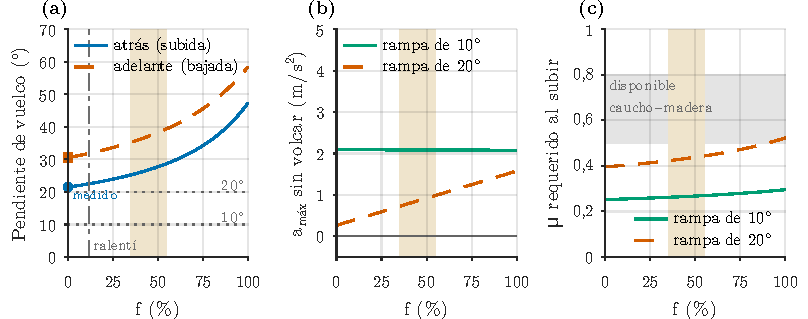
\includegraphics{figures/fig_rampa.pdf}
  \caption{Descarga de peso en la rampa frente a la fracción del peso del módulo sostenida por los rotores, $f$ ($f=0.5$ equivale a unos \SI{1540}{\micro\second} de colectivo). (a) Pendiente de vuelco estático hacia atrás (subida de frente) y hacia adelante (bajada de frente); los puntos son las pendientes medidas el 23/11 con el módulo trabado. (b) Margen de aceleración sin vuelco en 10 y \SI{20}{\degree}, con la inercia completa del módulo \eqref{eq:amaxf}. (c) Coeficiente de fricción que necesitan las ruedas motrices al subir, con la banda de caucho sobre madera. La franja ocre es la ventana propuesta de modo rampa.}
  \label{fig:rampa}
\end{figure}

\paragraph{3. Balance frente a un cardán}
La comparación honesta con un cardán ligero es la siguiente. Un cardán motorizado de \SI{1}{\kilo\gram} a la misma altura daría, con el mismo modelo, \SI{33.3}{\degree} de vuelco al subir sin gastar energía; el octocóptero solo lo supera con $f>0.72$. La ventaja del dron no es, por tanto, su masa, sino que su lastre es \emph{ajustable}: con $f=0$ carga las ruedas motrices para la tracción, con $f\approx0.5$ equilibra vuelco y tracción, y con $f=1$ desaparece de la base. Un cardán es un lastre fijo. A esto se suma que el octocóptero es el objeto de estudio del proyecto: un péndulo invertido con retardo de actuadores y autoridad de par limitada que se valida aquí, cautivo y con registros, antes del vuelo libre. El costo es doble: energía (Sección~\ref{sec:bateria}) y una banda de 0,2--\SI{0.3}{\hertz} en la que el octocóptero amplifica las aceleraciones de la base (Sección~\ref{sec:coupling}), que las rampas de referencia de la base deben evitar.

\paragraph{Lo que se ensayó y lo que falta}
Los recorridos por la rampa de \SI{10}{\degree} del 18/11 se hicieron con el firmware de banco y el colectivo en \SI{1300}{\micro\second} ($f\approx0.12$): el dron niveló la bandeja y descargó muy poco peso. La descarga es, por ahora, una predicción del modelo. Su validación necesita tres medidas: la corriente de la base con pinza amperimétrica, el ciclo de trabajo necesario para subir a velocidad constante con $f=0$ y $f=0.5$, y el ángulo al que la base empieza a levantar las ruedas omnidireccionales en una rampa variable.

\subsection{Margen de empuje y autonomía frente a la batería}
\label{sec:bateria}

El 20/11 el módulo despegó con las LiPo a 12,4\,V en reposo y, más tarde, con 11,1\,V ya no despegó. Esta sección explica el hecho y calcula el margen y la autonomía.

\paragraph{Modelo}
Cada ESC aplica al motor una fracción de la tensión de su rama, $V_{\mathrm{bus}}$. Con la hélice como carga, la velocidad del rotor es proporcional a esa tensión y el empuje a su cuadrado, así que, a orden fija,
\begin{equation}
  T=8k_F'\Big(\frac{V_{\mathrm{bus}}}{V_{\mathrm{ref}}}\Big)^2\Big(\frac{u-u_0}{860}\Big)^n ,
  \label{eq:tv}
\end{equation}
donde $k_F'$ es la ganancia identificada con la tensión $V_{\mathrm{ref}}$ de la Sección~\ref{sec:ident}. La tensión de la rama es la tensión en vacío de la LiPo, $V_{oc}$, menos la caída en la resistencia interna, el cable de \SI{1}{\metre} y los contactos (fusible, relé, XT60), $R_\Sigma$. Como la potencia de vuelo estacionario $P_b$ por rama es fija (el empuje es el peso), la corriente es $I_b=P_b/V_{\mathrm{bus}}$, y
\begin{equation}
  V_{\mathrm{bus}}=\tfrac12\Big(V_{oc}+\sqrt{V_{oc}^2-4R_\Sigma P_b}\Big).
  \label{eq:vbus}
\end{equation}
Igualando \eqref{eq:tv} al peso, el colectivo de despegue a otra tensión es
\begin{equation}
  u_{\mathrm{req}}=u_0+860\,x_{\mathrm{ref}}\Big(\frac{V_{\mathrm{bus,ref}}}{V_{\mathrm{bus}}}\Big)^{2/n},\qquad x_{\mathrm{ref}}=\frac{u_{\mathrm{ref}}-u_0}{860}=0.68\text{--}0{,}74,
  \label{eq:ureq}
\end{equation}
y con $n=1.6$ el colectivo crece con la potencia $1{,}25$ de la caída relativa de tensión. Los datos de entrada son: $P_b=\SI{250}{\watt}$ (tabla del A2212 con hélice 9450 de la auditoría, \SI{4.2}{\ampere} a 370\,gf con 11,1\,V, escalada con $T^{3/2}$ a 441\,gf por motor); $R_\Sigma=3r_c+\SI{22.6}{\milli\ohm}$, con $r_c=6$--\SI{15}{\milli\ohm} por celda [E] y un aumento del 50\% por debajo del 40\% de carga; y la curva típica tensión en reposo--estado de carga de una celda LiPo [E]. Las bandas de los resultados combinan los extremos de $k_F'$ y de $r_c$.

\paragraph{Resultados}
La Fig.~\ref{fig:bateria} y la Tabla~\ref{tab:bateria} dan el colectivo de despegue y la relación empuje/peso disponible frente a la tensión en reposo:
\begin{itemize}
  \item Con 12,4\,V (93\% de carga) la rama entrega \SI{22}{\ampere} a \SI{11.2}{\volt}. El módulo despega a 1725--\SI{1775}{\micro\second}: la orden \texttt{flotar} del firmware (\SI{1750}{\micro\second}) cae justo en esa banda. En el límite sostenido de \SI{1850}{\micro\second} la relación empuje/peso es 1,20--1,36, y en el máximo de \SI{1950}{\micro\second}, 1,48--1,68.
  \item Con 11,1\,V en reposo (12\% de carga) la tensión de la rama cae a \SI{9.3}{\volt} con \SI{27}{\ampere}, y el despegue exige 1850--\SI{2000}{\micro\second}: en el mejor caso, justo el límite sostenido, sin margen para el control de actitud; en el peor, más de lo que el ESC puede dar. Esto coincide con lo observado.
  \item La tensión mínima en reposo para despegar sin pasar de \SI{1850}{\micro\second} es 11,1--\SI{11.6}{\volt} (12--60\% de carga). Con la orden fija \texttt{flotar}, el módulo solo despega por encima de 12,05--\SI{12.1}{\volt}, y en el extremo pesimista de $k_F'$ no despega nunca.
  \item \textbf{Autonomía.} Desde 12,4\,V, el vuelo estacionario continuo dura 2,7--\SI{6.8}{\minute} hasta que el despegue exige \SI{1850}{\micro\second} (3,3--\SI{7.4}{\minute} desde 12,6\,V). El límite por energía con 80\% de descarga sería \SI{6.6}{\minute}. Lo que limita el vuelo es, por tanto, el margen de empuje y no la capacidad: solo se aprovecha la parte alta de la curva de descarga.
\end{itemize}

\begin{table}[!htbp]
\centering
\caption{Margen de empuje frente a la tensión en reposo de las LiPo (modelo \eqref{eq:vbus}--\eqref{eq:ureq}). Colectivo central con $u_{\mathrm{ref}}=\SI{1750}{\micro\second}$ y $r_c=\SI{10}{\milli\ohm}$; entre paréntesis, la banda.}
\label{tab:bateria}
\footnotesize
\setlength{\tabcolsep}{4pt}
\begin{tabular}{@{}cccccc@{}}
\toprule
$V_{oc}$ (V) & Carga (\%) & $V_{\mathrm{bus}}$ (V) & $I_b$ (A) & $u_{\mathrm{req}}$ (\si{\micro\second}) & Empuje/peso a \SI{1850}{\micro\second} \\
\midrule
12,6 & 100 & 11,45 & 21,8 & 1735 (1710--1760) & 1,24--1,42 \\
12,4 & 93 & 11,23 & 22,3 & 1750 (1725--1775) & 1,20--1,36 \\
12,2 & 84 & 11,00 & 22,7 & 1766 (1739--1793) & 1,14--1,31 \\
12,0 & 78 & 10,78 & 23,2 & 1782 (1754--1811) & 1,09--1,26 \\
11,8 & 68 & 10,55 & 23,7 & 1799 (1769--1831) & 1,04--1,21 \\
11,6 & 59 & 10,33 & 24,2 & 1817 (1786--1852) & 1,00--1,16 \\
11,4 & 40 & 10,10 & 24,8 & 1837 (1803--1875) & 0,95--1,12 \\
11,1 & 12 & 9,32 & 26,8 & 1910 (1850--2000) & 0,74--1,00 \\
\bottomrule
\end{tabular}
\end{table}

\begin{figure}[!htbp]
  \centering
  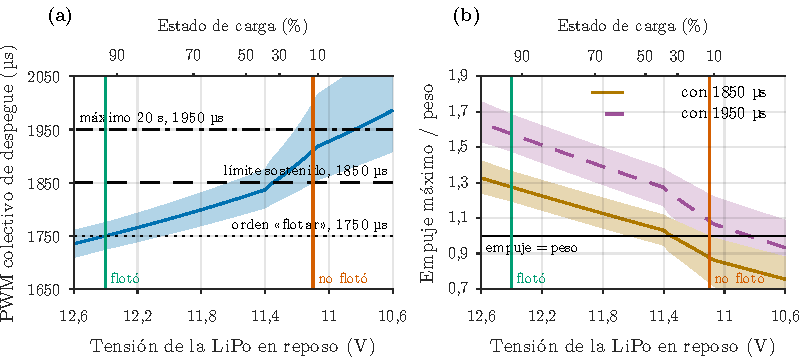
\includegraphics{figures/fig_bateria.pdf}
  \caption{Margen de empuje frente a la tensión en reposo de las LiPo. (a) Colectivo de despegue \eqref{eq:ureq}: línea central y banda por la incertidumbre de $k_F'$ y de la resistencia interna; líneas horizontales: orden \texttt{flotar}, límite sostenido y máximo del firmware v11; eje superior: estado de carga. (b) Relación empuje/peso disponible en el límite sostenido y en el máximo.}
  \label{fig:bateria}
\end{figure}

\paragraph{Contraste con los registros}
La carga que sacó cada batería en los vuelos 6--9 del 20/11, integrada a partir de las órdenes de motor registradas con el mismo modelo de potencia, fue 0,10, 0,22, 0,25 y \SI{0.44}{\ampere\hour} (\SI{1.0}{\ampere\hour}, el 31\% de la capacidad). Con ella, \eqref{eq:ureq} predice que el despegue del vuelo 9 necesitaba \SI{1787}{\micro\second} (banda 1758--\SI{1817}{\micro\second}); el registro muestra el despegue a \SI{1796}{\micro\second}, frente a \SI{1775}{\micro\second} en el vuelo 8. Al terminar el vuelo 9 el modelo da unos 11,6\,V en reposo, justo en el borde del límite sostenido. La lectura de 11,1\,V corresponde a una descarga mayor que la registrada: intentos posteriores sin registro o una medición hecha bajo carga o poco después de aterrizar, cuando la LiPo aún no se ha recuperado. Por eso el procedimiento de operación (Sección~\ref{sec:operation}) pide medir en reposo y registrar la tensión.

\paragraph{Consecuencias de diseño}
(i) El firmware debe leer VBAT\_A y VBAT\_B (los divisores ya están cableados en GPIO34/35; la auditoría recomienda pasar R2 y R4 a \SI{2.2}{\kilo\ohm} para quedar en la zona lineal del ADC, por debajo de \SI{2.45}{\volt}) y compensar el colectivo con \eqref{eq:ureq} como prealimentación, de modo que \texttt{flotar} signifique empuje igual al peso y no un pulso fijo. (ii) Conviene abortar la sesión cuando el despegue pida más de \SI{1825}{\micro\second}, para conservar margen de par. (iii) Las cuatro LiPo del grupo permiten dos sesiones de 3--\SI{7}{\minute} de vuelo continuo; el modo rampa de la Sección~\ref{sec:porquedron} cuesta mucho menos (2--5\% de carga por minuto) y es compatible con esa autonomía. (iv) Un cable de 12\,AWG reduce la caída del cable de \SI{0.34}{\volt} a unos \SI{0.2}{\volt}, lo que equivale a unos \SI{10}{\micro\second} de colectivo.
